\documentclass[a4paper,12pt,openright,oneside]{article}
%\usepackage[hmarginratio=3:2,vmarginratio=1:1]{geometry}
\usepackage[top=4cm,bottom=4cm,left=3cm,right=3cm]{geometry}
\usepackage{amsmath}
\usepackage{placeins}
\usepackage[font=footnotesize,labelfont={bf}]{caption}
\usepackage[font=footnotesize]{subcaption}
\usepackage{emptypage}
\usepackage{subdepth}
\usepackage{amssymb}
\usepackage{mathrsfs}
\usepackage[sort&compress]{natbib}
\usepackage{graphics}
\usepackage{fancyhdr}
\usepackage{graphicx}
\usepackage{braket}
\usepackage{epigraph}
\usepackage{bm}
\usepackage{multirow}
\usepackage[LGR,T1]{fontenc} % notice LGRx instead of LGR
\usepackage[utf8]{inputenc}   % utf8 is required
%\usepackage{textgreek}

\newcommand{\textgreek}[1]{\begingroup\fontencoding{LGR}\selectfont#1\endgroup}
\let\tmp\oddsidemargin
\let\oddsidemargin\evensidemargin
\let\evensidemargin\tmp
\reversemarginpar
\citestyle{nature}
\bibliographystyle{phjcp}
\linespread{1.2}

\newcommand*{\LargerCdot}{\raisebox{-0.25ex}{\scalebox{1.2}{$\cdot$}}}

\begin{document}
\cleardoublepage
\begin{titlepage}

\begin{center}
\linespread{1.3}
\textsc{\LARGE Approaching the Marangoni Effect through\\}
\textsc{\LARGE equilibrium molecular dynamics\\}
\vfill
\sc{H. G. A. Burton\\
Robinson College\\
Cambridge}

\vfill 


\includegraphics[width=0.3\textwidth]{Robinson_College_Crest.png}

\vfill 

\end{center}
\end{titlepage}

\cleardoublepage
%\newpage
\pagenumbering{roman}
\thispagestyle{empty}
\cleardoublepage
%\pagenumbering{roman}
\section*{Declaration}
\addcontentsline{toc}{section}{Declaration}

This dissertation is submitted in partial fulfilment of the requirements for Part III Chemistry. It describes work carried out in the Department of Chemistry in the Michaelmas Term 2015 and the Lent Term 2016. Unless otherwise indicated, the research described is my own and not the product of collaboration.
\\
\\
\\
\\
\\
\section*{Acknowledgements}
\addcontentsline{toc}{section}{Acknowledgements}

Acknowledgements will go here.

\newpage

\cleardoublepage
\thispagestyle{plain}
\addcontentsline{toc}{section}{Abstract}
\begin{center}
%\linespread{1.3}   
\textsc{\Large Holomorphic Hartree--Fock Theory:\\ From Formulation to Application}

    \vspace{0.2cm}
    \normalsize{{\textsc{Hugh Graham Alexander Burton}}}
    
\vspace{0.2cm}
    \normalsize{\textbf{Abstract}}
\end{center}
ABSTRACT GOES HERE

%\begin{abstract}
%The abstract goes here.
%\end{abstract}
\newpage

\tableofcontents
%\cleardoublepage
%\listoffigures
%\addcontentsline{toc}{chapter}{List of Figures}
%\cleardoublepage
%\listoftables
%\addcontentsline{toc}{chapter}{List of Tables}


\newpage
\cleardoublepage
\pagenumbering{arabic}
\fancyhead{}
\rhead{\thepage}
\lhead{\leftmark}
\lfoot[]{}
\rfoot[]{}
\cfoot[]{}
\fancypagestyle{plain}{
    \fancyhf{} % clear all header and footer fields
    \fancyhead{} % except the right top corner
    \renewcommand{\headrulewidth}{0pt} % remove line between header and main text
}
\pagestyle{fancy}
%\renewcommand{\chaptermark}[1]{\markboth{#1}{}}
%\renewcommand{\chaptermark}[1]{\markboth{\MakeUppercase{\chaptername}\ \thechapter. \ #1}{}}
%\renewcommand{\chaptermark}[1]{\markboth{\MakeUppercase{\chaptername} #1}{}}
%\renewcommand{\chaptermark}[1]{
%    \markboth{\MakeUppercase{
%            \chaptername\ \thechapter.
%\ #1}}{}}
%\renewcommand{\chaptermark}[1]{
%\markboth{\MakeUppercase{#1}}{}}
%\fancyhead[LO]{\leftmark}
%\fancyhead[RE]{\leftmark}
%fancyhead[LE,RO]{\thepage}
    
\newpage
\section{Introduction}
2015 saw the $160^{\mathrm{th}}$ anniversary of J. Thompson's first report\cite{JThompson} on the observation of flows occuring at a fluid--fluid interface as the result of a tangential chemical potential or temperature gradient.
This phenomenom was later termed the ``Marangoni Effet'' after it formed the basis of Carlo Marangoni's doctoral dissertation.\cite{Marangoni}
Since then temperature induced Marangoni flows, also known as thermocapillary flows, have been the subject of a number of studies and a macroscopic description has been developed through the works of Derjaguin\cite{SurfaceForces} and Levich\cite{Levich}, as summarised in the context of phoresis by Anderson\cite{Anderson}.

On the simplest level this effect can be described as a flow occuring due to a gradient in the surface--tension at the interface, with motion occuring from regions of low to regions of high surface--tenson.
However, this is not particulaly informative since the temperature dependence of surface--tension is itself known only through empirical studies.
Beyond a surface--tension based description, Derjaguin demonstrated that the flow can be calculated from the excess enthalpy of a fluid close to the interface, hence formulating a thermodynamic theory of thermocapillary motion.\cite{SurfaceForces}

The thermodynamic backbone upon which this theory is founded is reliant on knowledge of the macroscopic properties of the system.
In contrast, the flow itself is inherently a microscopic phenomenon acting in a localised way at the interfaces of bulk fluids. 
Such a localised effect cannot be faithfully described using a macroscopic thermodynamic description, instead it requires a microscopic theory formulated around the interpaticle interactions. 
No such theory currently exists, and there have been a very limited number of studies in this area.\cite{HolgerBoppHampe}
By studying the microscopic properties of a liqud--liquid interface, this report aims model the Maragnoni effect and investigate the link between these microscopic properties and the macroscopic fluid motion.

\subsection{Experimental studies}
Despite the lack of a microscopic theory, there has been substantial experimental research into the Marangoni effect.
Many of these studies have focussed on the more curious examples of Marangoni flows such as Thompson's ``tears of wine''\cite{JThompson,Venerus,Tadmor,Cazabat1995} and the ``coffee ring effect'',\cite{Sefian,HuLarson,Sefiane2014} whilst others have shown it is becoming ever more important in technological applications.
For example, Sternling and Scriven\cite{SternlingScriven} proposed Marangoni effects as the origin for interfacial turbelence and mass transport, yielding applications in fluid mixing and oil recovery,\cite{Aguilera2005,LyfordA,LyfordB} whilst Subramanian and Balasubramanian outline the importance of Marangoni forces for the motion of bubbles and droplets in reduced gravity environments.\cite{MotionOfBubblesAndDrops} 

In 1959, Young et al. produced a theoretical description of this motion of bubbles and droplets under the influence of a temperature gradient, a phenomena described as thermophoresis.\cite{Young1959}
They describe how the temperature gradient causes a higher surface--tension on the low temperature side of the droplet, resulting in a force pulling the surrounding fluid towards the low temperature region and a corresponding reaction force propelling the droplet towards the warmer fluid region (note the similarity to electrophoresis where there is no-net force within the droplet).
This force was measured experimentally by S. C. Hardy,\cite{Hardy1978} who used a temperature gradient to balance the Marangoni and buoyancy forces acting on a droplet within a fluid, thus holding the droplet stationary.
Later theoretical modelling by Kim and Subramanian suggested that the inclusion of surface--active substances could be used to prevent thermophoresis,\cite{KimSubramanianA,KimSubramanianB} a prediction that was later confirmed experimentally.\cite{BartonSubramanian,ChenStebe}

With the advances in space technology over the past half a century, thermophoresis and thermocapillary motion have become important mechanisms for fluid motion and mass transfer in low--gravity environments, where surface effects dominate over buoyancy driven motion.
The motion of bubbles and drops due to interfacial gradients is considered to be key for materials processing in space, enabling phase separation of binary mixtures and the potential to make uniform composite materials.\cite{BartonSubramanian}
Moreover, fluid transport in the absence of gravity is important for controlling fluid fuels aboard satellites, often carried for thrusters used to perform orbital adjustments.\cite{MotionOfBubblesAndDrops} 

\subsection{Striving for a microscopic description}
With so many potential applications, the search for a micrcoscpic description is becoming ever more significant and computer simulations are increasingly being used to understand this phenomenom.
Marangoni flows are inherently dynamic and must be studied using a time--dependent siumulation method such as Molecular Dynamics (henceforth MD).
To model the dynamic behaviour of an immiscible binary--mixture under the effect of a temperature gradient might initially appear trivial; simply create a temperature gradient for such a system and measure the expected flow velocity of the resulting particles.
This non-equilibirum approach is used by Hampe et al. in their study of the Marangoni effect.\cite{HolgerBoppHampe}
Despite their positive results, the method is complicated by the use of periodic boundary conditions (required to model a macroscopic fluid) that require each unit cell to have two temperature gradients such that the temperature is also periodic.
Any flow due to this gradient then generate an opposing concentration gradient and an equilibrium state will be reach where there is no fluid flow.

In this study we investigate the use of equilibirium molecular dynamics simulations for modelling the Marangoni effect.
Molecular dynamics heavily relies on the use of forces acting on a particle, these forces are calculated on each timestep and are used to integrate the equations of motion.
It is therefore easy to measure the stress acting on a fluid element during a simulation or to apply artificial forces.
By calculating the stress acting on a binary mixture at equilibrium for two different temperatures, the differential of the stress with respect to temperature can be estimated and used to infer a body force corresponding to the Marangoni force.
This force can then be applied as a constant body force in a non-equilibrium simulation on a fluid at an intermediate temperature to imitate the Marangoni force, thus circumventing the complications of a periodic temperature profile.
Finally, by measuring the velocity profile of this non--equilibrium simulation the Marangoni flow can be observed.

Using this equilibrium method we show that it is possible to calculate a Marangoni force at liquid--liquid interfaces from the fluid stress--tensor and use this force to generate the flow profile of the fluid.
We then use this technique to investigate the effect of surfactant molecules on the magnitude of the Marangoni forces and compare these results to the experimental observations.
Section 2 outlines the theoretical description of the Marangoni effect and the computational methods used are given in Section 3.
Sections 4 and 5 describe the simulations on binary--mixtures confined between two walls and periodic in three-dimension respectively and the effects of surfactants are investigated in Section 6.
Section 7 summarises the conclusions from the study and proposes directions for future investigations.

\newpage
\section{Theoretical Background}
\subsection{The macroscopic description}\label{Macroscopic}
The motion of fluids may be described macroscopically using the  Navier--Stokes equation.\cite{simpleLiquids} 
This models liquids as a continuous medium and combines the conservation of mass and momentum with the relation between the force on a volume element and the local fluid flow.
In the low Reynolds-number regime the flow velocity is small and the Navier--Stokes equation reduces to
\begin{equation}
\label{NavierStokes}
\eta \nabla^{2}\mathbf{\nu}(r,t) = \nabla P(r,t) - \mathbf{f}(r).
\end{equation}
Equation \ref{NavierStokes} shows that motion in fluids \textit{can only} occur under the presence of a pressure gradient or external forces.
In the case of Marangoni flows, motion due to the temperature gradient must result from induced local pressure gradients, which may be derived from thermodynamics.

Consider a binary--mixture with an interface at $z=0$.
The Gibbs--Duhem equation gives
\begin{equation}
V \mathrm{d}P = \sum_{i=0}^{n} N_{i} \mathrm{d}\mu_{i} + S \mathrm{d}T.
\end{equation}
The bulk fluid pressure is constant and isotropic, giving
\begin{equation}
\label{GibbsDuhem}
\left( \frac{\partial P}{\partial x}\right) = \sum_{i=0}^{n} \rho_{i}^{\mathrm{B}} \left(\frac{\partial \mu_{i}}{\partial x}\right) + \frac{S}{V} \left( \frac{\partial T}{\partial x}\right) = 0.
\end{equation}
The Maxwell relations relate the entropy to the partial differential of chemical potential with respect to temperature through
\begin{equation}
\left( \frac{\partial\mu_{i}}{\partial T} \right)_{P,N_{i}} = - \left(\frac{\partial S}{\partial N_{i}}\right)_{P,T}.
\end{equation}
The total entropy is the weighted sum of the partial entropy of the species in the system, 
\begin{equation}
S = \sum_{i=0}^{n}s_{i}N_{i},
\end{equation}
thus
\begin{equation}
\left( \frac{\partial\mu_{i}}{\partial T} \right)_{P,N_{i}} = - s_{i}.
\end{equation}
\\
This allows Equation \ref{GibbsDuhem} to be expressed as
\begin{equation}
\left( - \sum_{i=1}^{n}\rho_{i}^{\mathrm{B}}s_{i}^{\mathrm{B}}+\frac{S^{\mathrm{B}}}{V}\right)\left(\frac{\partial T}{\partial x}\right) = 0,
\end{equation}
for which the solution is 
\begin{equation}
\frac{S^{\mathrm{B}}}{V} = \sum_{i=1}^{n}\rho_{i}^{\mathrm{B}}s_{i}^{\mathrm{B}}.
\end{equation}
\\
Consider the case close to an interface or surface where the pressure will deviate from its bulk value.
Since $\mu_{i}$ and T are independent of $z$,
\begin{equation}
\left(\frac{\partial \mu_{i}}{\partial T}\right) = - s_{i}^{\mathrm{B}},
\end{equation}
and the pressure gradient reduces to
\begin{equation}
\left(\frac{\partial P(z,x)}{\partial x}\right) = \left(\sum_{i=1}^{n}\rho_{i}(z)\left(s_{i}(z)-s_{i}^{\mathrm{B}}\right)\right)\left(\frac{\partial T}{\partial x}\right).
\label{PressGrad}
\end{equation}

For an ideal mixture, the partial entropy is given by $s_{i}=\frac{1}{T} \left(\mu_{i}-h_{i} \right)$, and thus Equation \ref{PressGrad} can be expressed in terms of the excess enthalpy density, $\Delta h(z)$,
\begin{equation}
\label{ExcessEnthalpy}
\left(\frac{\partial P(z,x)}{\partial x}\right)= - \Delta h(z)\frac{1}{T} \left( \frac{\partial T}{\partial x} \right) 
= - \Delta h(z) \left( \frac{\partial \ln T}{\partial x} \right).
\end{equation}

Substituting Equation \ref{ExcessEnthalpy} into Equation \ref{NavierStokes} and assuming there is no pressure gradient in the $z$ or $y$ direction allows the velocity, $v(z)$, at the interface to be computed as
\begin{equation}
\label{DoubleIntegral}
v (z=0) = - \frac{1}{\eta}\int_{0}^{\infty} \mathrm{d}z\, z \Delta h(z) \frac{\partial T}{\partial x}
\end{equation}
where it has been assumed that the fluid in the bulk is at rest ($v_{x}(z=\infty)=0$) is at rest.
This expression is almost equivalent to that derived by Derjaguin et. al., except for a factor of two, suggesting there may be an error in Derjaguin's approach.\cite{SurfaceForces, Anderson}

\subsection{A microscopic approach}
The Marangoni effect is a phenomenon occurring on microscopic length--scales, and hence this macroscopic hydrodynamic approach is not entirely appropriate.
Instead of solving the Navier--Stokes equation, the velocity should be related directly to the local forces acting on the fluid, which may be calculated from the local stress tensor,
\begin{equation}
\label{ForceStress}
f_{x}(z) = - \left( \frac{\partial \sigma_{xx}(z,x)}{\partial x} \right).
\end{equation}

In the case of Marangoni flows, the force is due to a temperature gradient and $f_{x}(z)$ can be calculated from the chain rule as
\begin{equation}
\label{ForceStressTemp}
f_{x}(z) = - \left( \frac{\partial \sigma_{xx}(z,x)}{\partial T} \right) \left( \frac{\partial T}{\partial x} \right).
\end{equation}

\subsection{The Finite Difference Approach}
Equation \ref{ForceStressTemp} shows that the force due to a temperature gradient can be inferred from the temperature variation of the stress tensor. 
To first order, the temperature gradient of the stress tensor can be calculated using a finite difference approach as
\begin{equation}
\label{FinDiff}
\left( \frac{\partial \sigma_{xx}(z,x)}{\partial T} \right) \approx \frac{\sigma_{xx}^{T_{2}}(z,x) - \sigma_{xx}^{T_{1}}(z,x)}{T_{2} - T_{1}}.
\end{equation}
Using this approximation, the Marangoni flow profile can be computed as follows:
\begin{enumerate}
	\item Compute $\sigma_{xx}(z)$ for an equilibrium system at a given temperature $T_{1}$.
	\item Repeat the calculation for another equilibrium system at a slightly higher temperate $T_{2}$.
	\item Approximate the partial derivative of the transverse stress with respect to temperature using the finite difference, Equation \ref{FinDiff}.
	\item Infer $f_{x}(z)$ for a specified value of $\partial T / \partial x$ using Equation \ref{ForceStressTemp} to calculate a force profile.
	\item Compute the flow profile by applying $f_{x}(z)$ as an artificial body force to an equilibrium simulation at an intermediate temperature $T_{3}$ (where $T_{1} < T_{3} < T_{2}$).
\end{enumerate}

\subsection{Non-uniqueness of the pressure tensor}
The stress tensor is intimately related to the pressure tensor through
\begin{equation}
\sigma_{\alpha \beta}(\mathbf{r}) = - P_{\alpha \beta} (\mathbf{r}).
\end{equation}
The pressure tensor is composed of a kinetic contribution, arising from the momentum transfer of particles on the container walls, and a potential contribution attributed to the interparticle forces.\cite{VarnikBinder}
The kinetic part may be calculated from the ideal gas contribution,
\begin{equation}
\mathbf{P}^{K}(\mathbf{r})=k_{\mathrm{B}} T \rho(\mathbf{r}) \hat{\mathbf{I}},
\end{equation}
whilst the potential contribution cannot be uniquely defined.

For a homogeneous fluid the stress tensor is isotropic, with each diagonal element equal to $- P$, where $P$ is the bulk hydrostatic pressure. 
This pressure can be calculated using the Virial equation, originally derived from the Virial theorem of Clausius\cite{Clausius}, (although also derivable by differentiating the canonical partition function\cite{MolTheoryCap}) to give
\begin{equation}
\label{VirialPressure}
P_{\alpha \beta}(\mathbf{r})=\frac{1}{V} \left( -m(\mathbf{r})\left< \nu_{\alpha} \nu_{\beta} \right> + \frac{1}{2} \sum_{i}^{N} \sum_{j \neq i}^{N} (r_{\alpha}^{(i)} - r_{\alpha}^{(j)})f_{\beta}^{ij} \right).
\end{equation}
Clausius' formulation calculates the local pressure by considering the forces acting on particles located within a volume element at $\mathbf{r}$.

In an inhomogeneous system there is an ambiguity over which particles should contribute to the force at a given position.\cite{MolTheoryCap,VarnikBinder,Rowlinson1982}
This was first reported by Irving and Kirkwood\cite{IrvingKirkwood1949,IrvingKirkwood1950} who describe an alternative method that computes the pressure tensor from the forces acting across an infinitesimal surface $\mathrm{d}\mathbf{A}$ located at $\mathbf{r}$.
They calculate the local pressure tensor using only pairs of particles for which the line connecting their centers of mass passes through $\mathrm{d}\mathbf{A}$.
For planar systems, such as those involving an interface in the $(x,y)$ plane, the pressure tensor depends only on the distance from this interface and the normal and tangential components can be expressed as
\begin{align}
\label{IKpressureN}
P_{\mathrm{N}}^{\mathrm{IK}}(z) &= \rho(z)k_{\mathrm{B}}T-\frac{1}{2A} \left< \sum_{i \neq j} \frac{|z_{ij}|}{r_{ij}} U'(r_{ij}) \Theta \left( \frac{z-z_{i}}{z_{ij}}\right) \Theta \left( \frac{z_{j} - z}{z_{ij}} \right) \right>,\\
\label{IKpressureT}
P_{\mathrm{T}}^{\mathrm{IK}}(z) &= \rho(z)k_{\mathrm{B}}T-\frac{1}{4A} \left< \sum_{i \neq j} \frac{x^{2}_{ij} + y^{2}_{ij}}{r_{ij}} \frac{U'(r_{ij})}{|z_{ij}|} \Theta \left( \frac{z-z_{i}}{z_{ij}}\right) \Theta \left( \frac{z_{j} - z}{z_{ij}} \right) \right>.
\end{align}

The Irving--Kirkwood stress has key advantages over the Virial method for studying confined systems, in particular it yields a normal component independent of local fluctuations in the number density.
Density fluctuations occur close to walls due to structural layering of the fluid, and there is reduced density at liquid--liquid interfaces from the finite width of the interfacial region.
As a result, oscillations in the normal component of the Virial pressure are observed in such systems\cite{VarnikBinder} whilst the Irving--Kirkwood pressure yields a constant normal component, equal to the bulk hydrostatic pressure.
This is more consistent with the expected result since the fluid is isotropic in the direction normal to the surface.

\newpage
\section{Computational Methods}

Equilibrium molecular dynamics simulations of a symmetric binary--mixture of partially miscible fluids were used to measure the stresses acting on the fluid at two different temperatures.
The Marangoni force was then inferred using Equation \ref{FinDiff}.
Where possible, this force was applied as an artificial body force in a simulation at an intermediate temperature to generate a Marangoni flow profile.

Two key systems were studied, a symmetric binary–mixture under three--dimensional periodic boundary conditions, and a binary--mixture periodic in the $(x,y)$ plane but confined between two walls in the $z$--dimension, as shown in Figure \ref{SetUp}.
All molecular dynamics simulations were executed using the LAMMPS (Large Atomic and Molecular Massively Parallel Simulator) package.\cite{LAMMPS}  
g
\begin{figure}[h]
	\begin{subfigure}{.5\linewidth}
		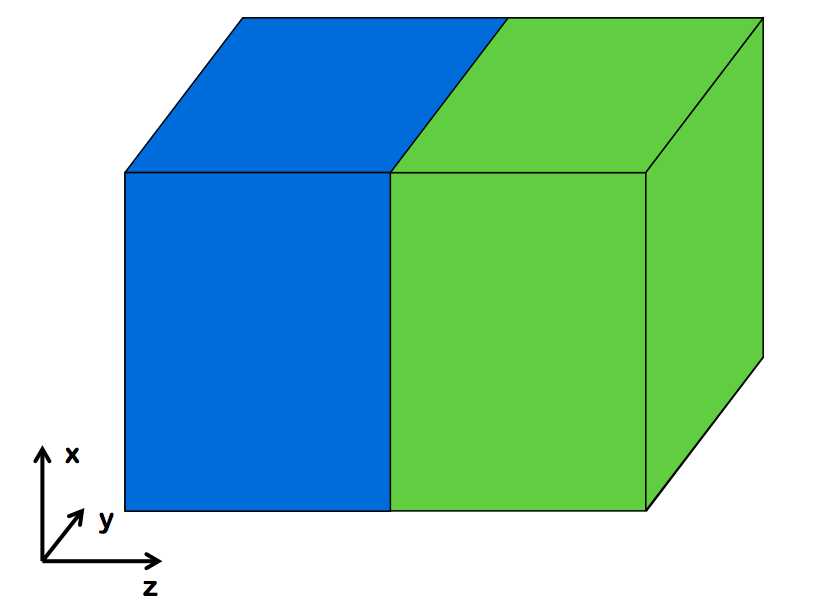
\includegraphics[scale=0.25]{AABB.png}
		\caption{Binary--mixture periodic in all dimensions}
		\label{AABB}
	\end{subfigure}
	\begin{subfigure}{.5\linewidth}
		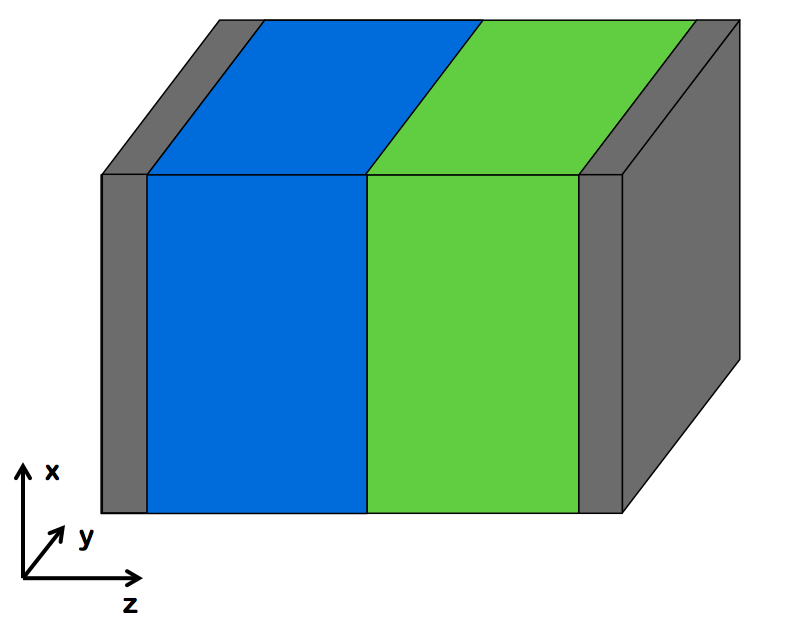
\includegraphics[scale=0.25]{AABB_piston.png}
		\caption{Binary--mixture confined by planar walls} 
		\label{AABB_piston}
	\end{subfigure}
	\caption{Both the systems studied incorporated a partially miscible binary--mixture of Fluid A (blue) and Fluid B (green).
For the mixture periodic in all dimensions, the pressure is regulated using a Nos\'{e}--Hoover barostat.
In the confined fluid, the walls are used to create a piston and an external force equal to $P_{\mathrm{ext}} \times A_{\mathrm{wall}}$ is applied.
}
	\label{SetUp}
\end{figure}

\subsection{Interaction Model}\label{InteractionModel}
The fluids were modelled using spherical particles and their interaction was tuned to a pair--wise truncated Lennard--Jones potential:
\begin{equation}
V \left( \mathbf{r}^{\mathrm{N}} \right) = \frac{1}{2} \sum_{i\neq j} \phi \left( r_{ij} \right)
\end{equation}
where
\begin{align}
\label{LJ}
\phi \left( r_{ij} \right) &= 4 \epsilon_{ij} \left( \left( \frac{\sigma_{ij}}{r_{ij}}\right)^{12} - \left( \frac{\sigma_{ij}}{r_{ij}}\right)^{6} \right)\ \mathrm{for}\ r \leq r_{c}\\
\phi \left( r_{ij} \right) &= 0\ \mathrm{for} r > r_{c}.
\end{align}
This potential involves an attractive $r_{ij}^{-6}$ term accounting for the long--range Van der Waal's interaction and a short--range $r_{ij}^{-12}$ repulsive term corresponding to the Pauli repulsion between particles.
The length--scale of the potential is given by $\sigma_{ij}$ (chosen to be equal for all pairs of $i$ and $j$) whilst the parameter $\epsilon_{ij}$ determines the strength of the interaction. 

The miscibility of the two fluids (A and B) can be controlled using the relative values of the interaction parameter; in this study the values chosen were:
\begin{align}
\epsilon_{A,A} &= \epsilon_{B,B} = 1.0,\\
\epsilon_{A,B} &= 0.55,
\end{align}
in agreement with previous studies on similar Lennard--Jones binary--mixtures.\cite{MorenzoRazo,Blas,HolgerBoppHampe}
The cutoff for the potential was chosen to be $r_{c} = 4\ \sigma$.

\subsection{Reduced Units}\label{ReducedUnits}
Physical quantities including distances and energies are expressed in terms of reduced units.
For a Lennard--Jones system, the basic units are $\sigma$ for length, $\epsilon$ for energy and $m$ for mass, from which all other units may be derived.\cite{FrenkelSmit}
Physical quantities become dimensionless when expressed in terms of these units, for example $r^{*} \equiv r / \sigma$.
Scaled coordinates expressed relative to the simulation box size are also used, for example $z' = z^{*} / L_{z^{*}}$ where $L_{z^{*}}$ is the dimension of the box in the z--direction.
These are useful if the box--dimensions vary, such as when a barostat acts on the system.

\subsection{Thermostats}\label{Thermostats}
In molecular dynamics simulations, the temperature is controlled using thermostats, which simulate the coupling of the system to an external heat bath.

Thermostats work by applying a stochastic frictional force to particles, either by adding a random force to momenta (Langevin)\cite{Langevin} or reassigning the velocity of randomly chosen particles to that obtained from the Maxwell distribution (Anderson)\cite{AndersonTherm}.
The Nos\'{e}--Hoover thermostat was used throughout this study.
This introduces a fictitious frictional force into the equations of motion which adjusts the particle velocities until the temperature is equal to the desired value.\cite{NoseHoover1, NoseHoover2, NoseHoover3}
The equations of motion in 3D become:
\begin{align}
m_{i}\frac{\mathrm{d}^{2}\mathbf{r}_{}}{\mathrm{d} t ^{2}} =& \mathbf{f}_{i} - \zeta m_{i} \mathbf{v}_{i}\\
\frac{\mathrm{d} \zeta (t)}{\mathrm{d} t} =& \frac{1}{Q}\left[ \sum_{i=1}^{N} m_{i} \frac{\mathbf{v}^{2}_{i}}{2} - \frac{3N+1}{2}k_{\mathrm{B}}T\right].
\end{align}
The result is a system where the energy fluctuates but the combined energy of the system and heat bath remains constant, maintaining a canonical ensemble.

\subsection{Barostats}\label{Barostats}
The bulk pressure of the fluid must also be held constant.
A piston provides the simplest method and is relatively easy to create; the fluid is confined between two solid walls and a force equal to $P_{ext} \times A_{wall}$ is applied.
This was used for studying the binary--mixture confined between two walls.
In the case of Marangoni flows, a thermocapillary effect will also occur at the boundary of the liquid and the solid piston.
The interface must be sufficiently far from the walls such that this thermocapillary force can be ignored.
Only the interfacial force should then be applied in the final simulation.

Alternatively a Nos\'{e}--Hoover barostat can regulate the pressure by adjusting the simulation box dimensions and altering the equations of motion accordingly. \cite{NoseHoover1, NoseHoover2, NoseHoover3}
When studying surface effects, the box size must only be changed in the direction perpendicular to the interface, since any other direction will alter its area and create an error in the thermodynamic pressure,
\begin{equation}
P = - \left( \frac{\partial F}{\partial V} \right)_{T} + \gamma \left( \frac{\partial A}{\partial V} \right)_{T}.
\end{equation}

\subsection{Preparing the system}\label{SystemPrep}
The fluid was prepared from a face--centred cubic lattice with a spacing of $1.64414\ \sigma$ and a simulation box size of $L_{x^{*}}=13.1531$, $L_{y^{*}}=13.1531$ and $L_{z^{*}}=32.8828$.
This lattice was melted over $2\times 10^{6}$ timesteps of length $0.001\ \tau$ to generate a fluid state.
The barostat was set to a pressure of $P^{*} = 0.1$ and the temperatures used were $T^{*} = 0.8$ and $T^{*} = 0.9$, ensuring the system occupied the liquid region of the Lennard--Jones phase space.\cite{Smit}
Solid walls in the system were constructed with a harmonically bonded lattice using a spring constant of $K^{*} = 2500$ and an equilibrium bond length of $r^{*}_{0}=1.163$.

\subsection{Calculating the stress tensor}\label{CalcStress}
The Virial stress tensor was calculated using an in--built function within the LAMMPS package, which returns the stress tensor for each atom.
However, LAMMPS does not have a method for calculating the Irving--Kirkwood stresstensor.
Instead this was calculated by dumping the particle positions on a given timestep to a file and post--processing.
The stress tensor was then computed using a programme written by R. Ganti and adapted for the specific systems studied.
Since the Virial method is implemented in parallel whilst the Irving--Kirkwood method is not, the Irving--Kirkwood stress was significantly more expensive to compute, incurring approximately a 4-fold increase in computational time.

\subsection{Computing averages}\label{ComputeAve}
Usually time--averages of physical observables are calculated in molecular dynamics simulations. 
In the systems studied, the observables are the number density, stress tensor and particle velocities.
Their values were measured every timestep and spatially averaged for $400$ planar slabs across the z--dimension of the box.
These spatial averages were then time--averaged over the full duration of the simulation.

Under the ergodic hypothesis, time--averages can be equated to ensemble averages for an infinitely long simulation time.\cite{Bopp2008}
Practically, however, these averages must be evaluated over a finite time period and have an associated statistical error.
The method of block--averaging, developed by Flybjerg and Peterson, provides an efficient technique for computing this error.\cite{Flyvbjerg1989}
They show that the variance of an observable, $A$, can be estimated by
\begin{equation}
\mathrm{var}(A) \geq \left< \frac{C_{0}}{n-1} \right>,
\end{equation}
where $C_{0}$ is the value of the time-correlation function for the block--transformed data at $t=0$ and is given by
\begin{equation}
C_{0} \equiv \frac{1}{n} \sum_{k=1}^{n} \left( A_{k} - \bar{A} \right) \left(A_{k} - \bar{A} \right).
\end{equation}
A lower bound for the variance can be calculated by finding the block length at which this estimate reaches a plateau.
Furthermore, the error in the variance can be estimated as 
\begin{equation}
\sqrt{\frac{2}{n-1} \times \frac{C_{0}}{n-1}}.
\end{equation}

\begin{figure*}[h]
\hspace{-3em}
	\begin{subfigure}{.5\linewidth}
                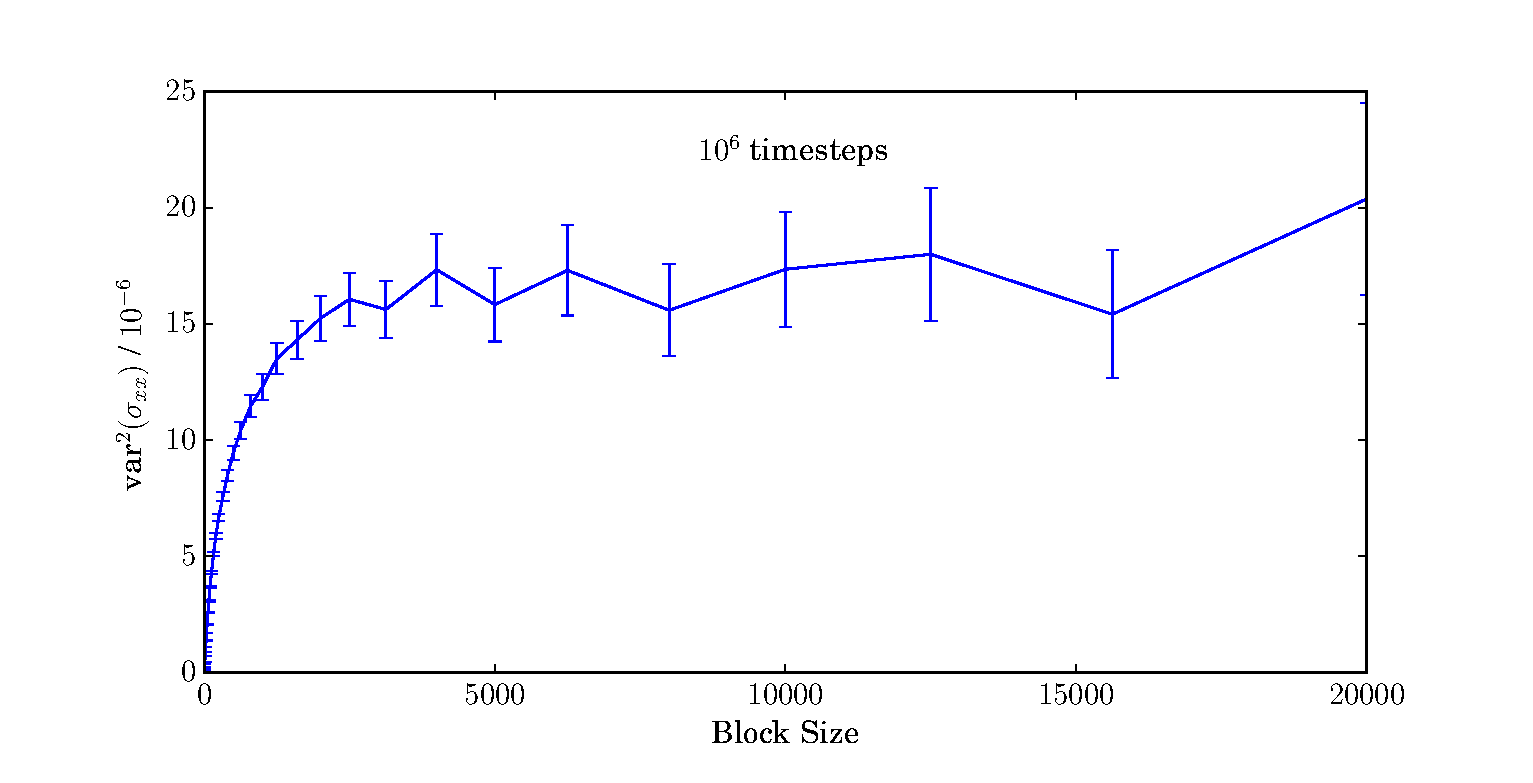
\includegraphics[scale=0.6]{block_average_1e6.eps}
                \caption{Simulation time = $1000\ \tau$}
        \end{subfigure}
\hspace{2em}
        \begin{subfigure}{.5\linewidth}
                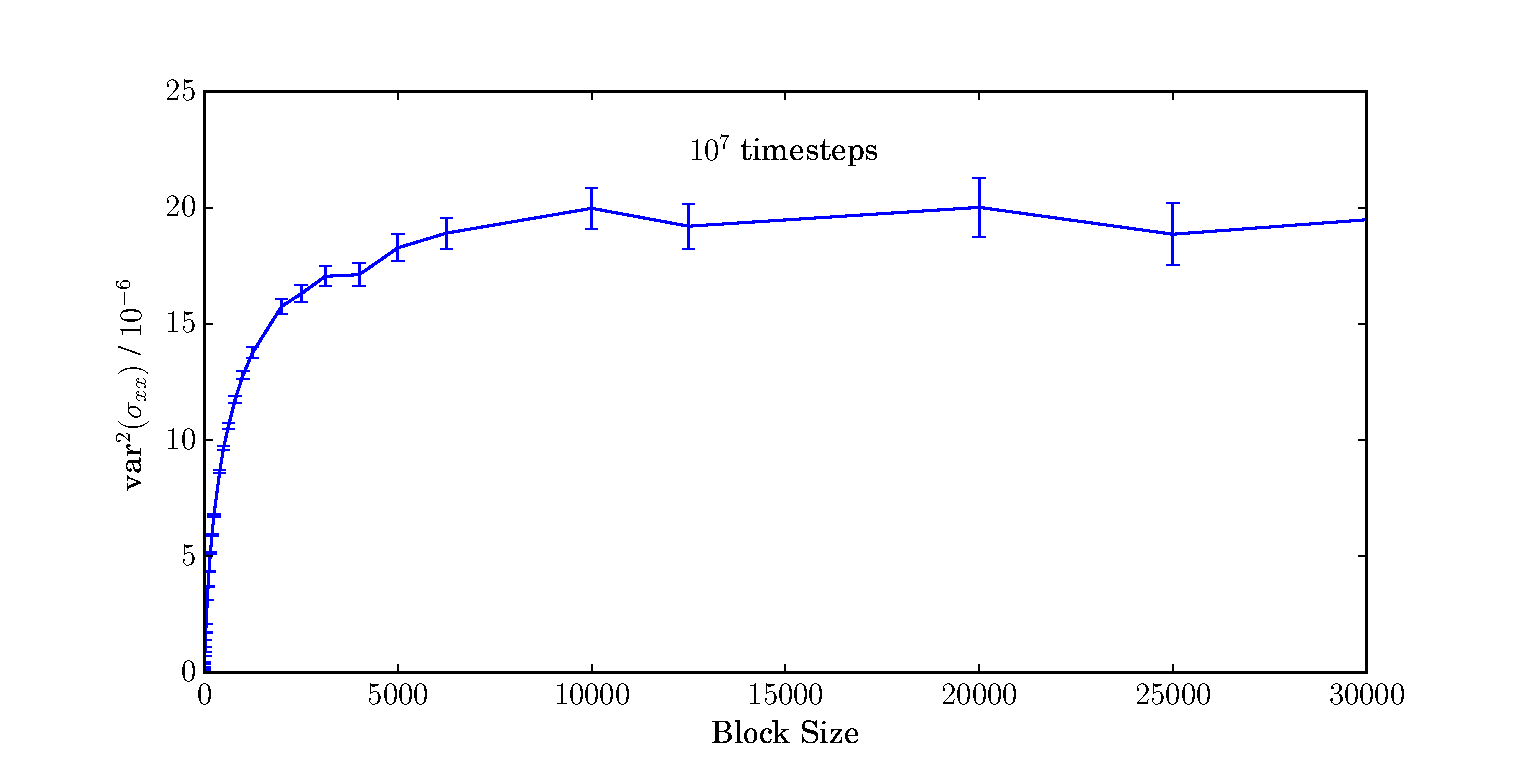
\includegraphics[scale=0.6]{block_average_10e6.eps}
                \caption{Simulation time = $10000\ \tau$}
	\end{subfigure}
	\caption{The blocking analysis for a system identical to those studied is compared for simulation times of $1000\ \tau$ and $10000\ \tau$.
Plateaus in the estimate of the variance begin at block lengths of approximately $5\ \tau$ and $10\ \tau$ respectively.
The error in the variance does not become significant until much larger block lengths.
Throughout the subsequent simulations, a block size of $10\ \tau$ was used.
This ensured decorrelation of the data and produced a reliable estimate of the statistical error.
}
\label{blocking}
\end{figure*}

A blocking--analysis for a binary--mixture identical to those used throughout this study was executed over a simulation time of $1,000\ \tau$ and $10,000\ \tau$, as shown in Figure \ref{blocking}.
The plateau begins at a block length of $10\ \tau$ for the long simulation and $5\ \tau$ for the shorter run, with little increase in the error of the variance until a much larger block size.
Considering this result, a block length of $10\ \tau$ was used to provide a good estimate for the error of all time--averages calculated in the subsequent simulations.
\FloatBarrier

\subsection{Modelling surfactant molecules}\label{ModellingSurfactants}
\begin{figure*}[h]
\centering
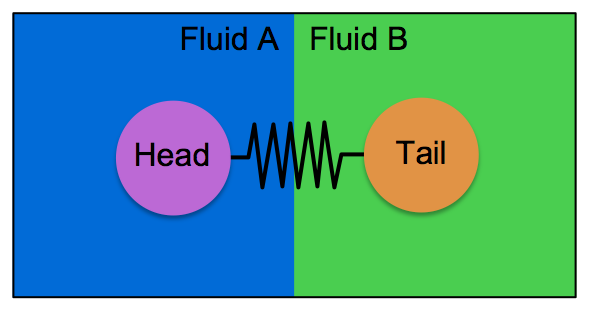
\includegraphics[scale=0.4]{surfactant.png}
\caption{Surfactant molecules are represented by a pair of spherical Lennard--Jones particles connected by a harmonic bond. 
The head particle has a stronger interaction with Fluid A ($\epsilon_{H, A} = 1.33$ and $\epsilon_{H, B} = 0.17$) whilst the tail has a stronger interaction with Fluid B ($\epsilon_{T, A} = 0.17$ and $\epsilon_{T, B} = 1.33$).
This generates the desired surface active behaviour.
 }
\label{surfactant}
\end{figure*}
To investigate the effects of surfactants on the Marangoni effect, the surfactant molecules were modelled as a pair of Lennard--Jones particles connected by a harmonic bond with spring constant $K^{*} = 25$ and equilibrium bond length $r^{*}_{0}=1.63$.
Inspired by Howes and Radke's study on non--ionic surfactants,\cite{HowesSurfactant} the `head' particle has a stronger interaction with Fluid A particles, ($\epsilon_{H, A} = 1.33$ and $\epsilon_{H, B} = 0.17$) whilst the `tail' particle has a stronger interaction with Fluid B particles ($\epsilon_{T, A} = 0.17$ and $\epsilon_{T, B} = 1.33$).
The `head' and `tail' groups interact with each other with strength $\epsilon_{H, T} = 1.00$.
\FloatBarrier

\subsection{Software details}\label{SoftwareDetails}
All molecular dynamics simulations were carried out using the LAMMPS (Large Atomic and Molecular Massively Parallel Simulator) package.\cite{LAMMPS}
Additional processing was carried out using Numpy.\cite{NumPy}
All graphical figures were plotted using Matplotlib.\cite{MatPlotLib}


\newpage
\section{Results and Discussion}
\subsection{Binary--mixture confined between two walls}\label{Piston}
Initially, a binary--mixture of two fluids confined between two walls was studied. 
The fluid was prepared as described in Section \ref{SystemPrep} at a pressure of $P^{*} = 0.1$ and temperatures of $T^{*} = 0.8$ and $T^{*} = 0.9$.
The confining walls were used as a piston to control the pressure.

\subsubsection{Using the Virial stress}\label{VirialStressPiston}
Once equilibrated, the simulations were run for $40 \times 10^{6}$ timesteps of length $0.001\ \tau$ and the number density and Virial stress tensor were computed every timestep.
These values were then time-averaged to produce profiles for the number density and $\sigma(z')$ as shown in Figures \ref{PisVirRho} and \ref{PisVirStress}. 

\FloatBarrier
\begin{figure*}[h]
\centering
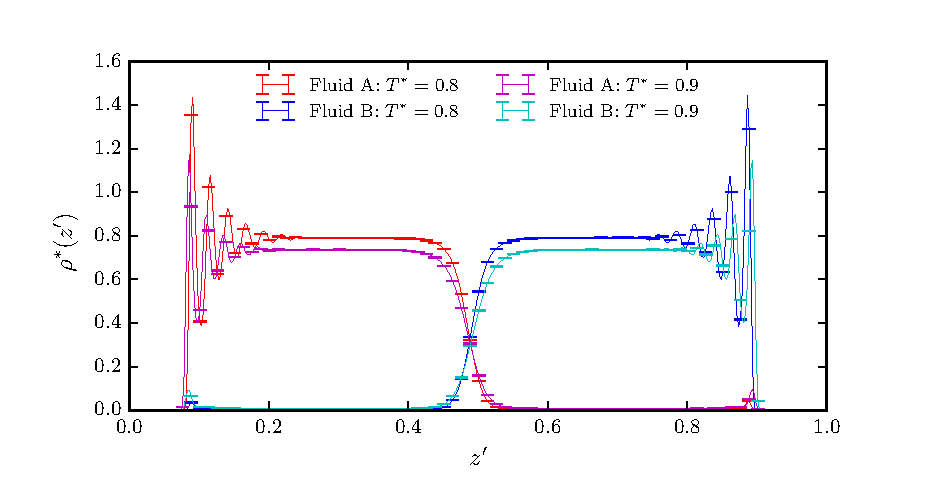
\includegraphics[scale=1.0]{PisVirRho}
\caption{The number density for the two fluids confined between two walls at $T^{*} = 0.8$ and $T^{*} = 0.9$ was time--averaged over $40 \times 10^{6}$ timesteps of length $0.001\ \tau$. 
The bulk density is uniform, representing a fluid state, and the interface manifests itself as a sharp change in the densities of the two fluids.
Structural layering of the fluid creates oscillations in the density close to the walls.
}
\label{PisVirRho}
\end{figure*}

\begin{figure*}[h]
\centering
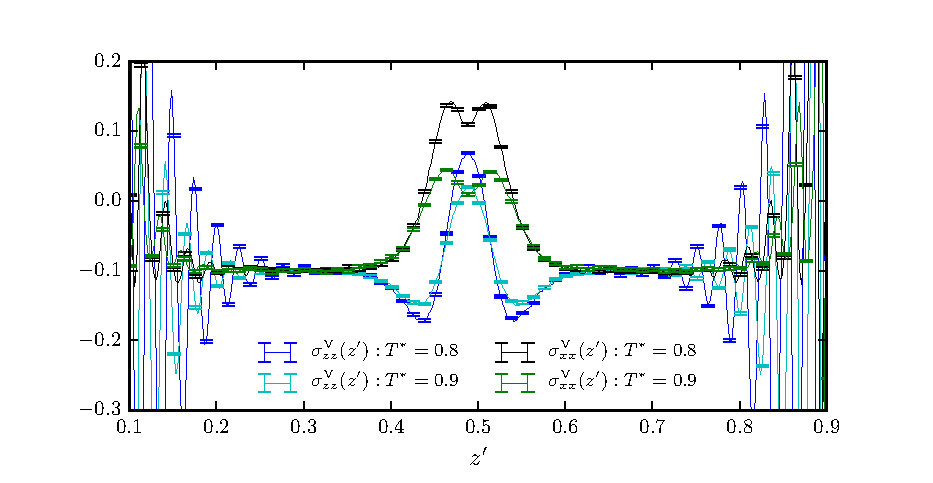
\includegraphics[scale=1.0]{PisVirStress}
\caption{The Virial stress tensor components for the combined fluid confined between two walls at $T^{*} = 0.8$ and $T^{*} = 0.9$ was time--averaged over $40 \times 10^{6}$ timesteps of length $0.001\ \tau$.
Both the normal and tangential stress show bulk values equal to $-P_{ext}$, representing the hydrostatic pressure.
There is a peak in the tangential stress at the interface due to the anisotropy of the interparticle forces in this region.
This can be related to the surface tension and its temperature dependence is the driving force for the Marangoni effect.
There is also a change in the normal component at the interface, resulting from the dependence of the Virial stress on density deviations.
Towards the wall there are temperature dependent oscillations in both components which provide the origin of the thermophoretic force.
}
\label{PisVirStress}
\end{figure*}

Both the density profile and the stress profile show the expected features of a binary--mixture. 
There is a uniform density in the bulk of the fluid and an interfacial region of finite width where the density of one species falls sharply and the density of the other increases.
Close to the walls, there are large oscillations in the density as a consequence of structural layering in the fluid close to the solid.

For the stress profile, the bulk values for the normal and tangential components are equal to $-P_{\mathrm{ext}}$, corresponding to the hydrostatic pressure of the fluid as expected.
At the interface there is a peak in the tangential stress due to the anisotropy of the intermolecular forces in this region; this can be related to the interfacial tension.\cite{Marchand2011}
Furthermore, there is a change in the normal component at the interface, resulting from dependence of the Virial stress on density deviations in this region.

The time--averaged values for the stress were then used to estimate the derivative of the tangential stress with respect to temperature using Equation \ref{FinDiff}, as shown in Figure \ref{PisVirForce}.
This derivative shows a peak at the interface of the two fluids, providing the origin of the Marangoni force.
In the bulk of the fluid the derivative is zero within statistical error, ensuring there is no force acting in this region.
In addition, the derivative oscillates at the surface of the wall.
This can be interpreted as a thermophoretic force and is henceforth ignored.

\begin{figure*}[h]
\centering
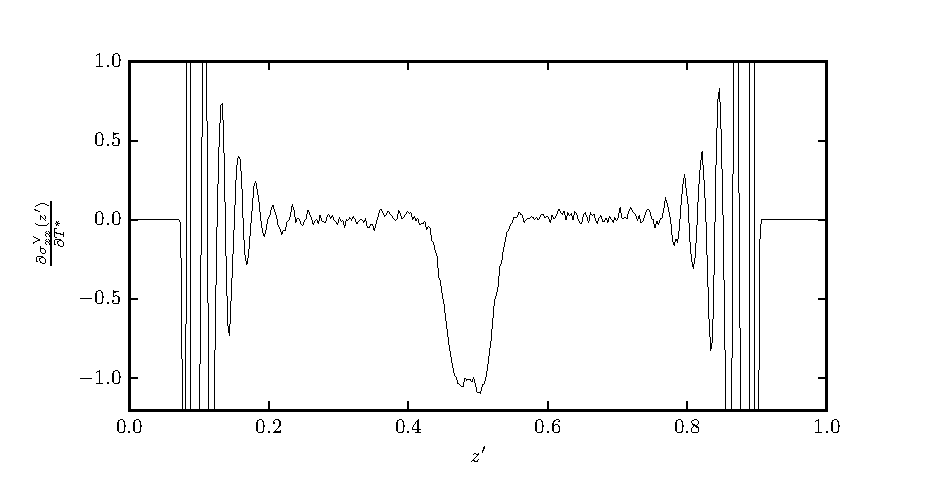
\includegraphics[scale=1.0]{PisVirForce}
\caption{The derivate of the tangential component of the Virial stress with respect to temperature, calculated using the finite difference approximation, shows a negative peak at the interface.
When combined with a specified temperature gradient, this generates a force in the opposite direction to a temperature gradient, imitating the Marangoni force.
The oscillations at the liquid--solid surface create the thermophoretic force and are subsequentlyignored.}
\label{PisVirForce}
\end{figure*}
\FloatBarrier

Using the central $1/3$ of the derivative profile and a temperature gradient of $\partial T^{*} / \partial x^{*} = 0.001$, an artificial Marangoni force was computed through Equation \ref{ForceStressTemp}.
This force was applied to an identical system prepared at $T^{*} = 0.85$.
An equilibrium simulation was then run for $40 \times 10^{6}$ timesteps and the time--average of the x--component of the fluid velocity, $v^{*}_{x}(z')$, was computed.
The momenta of the walls in the $x,y$ plane were fixed such that they provided a stationary reference point for the fluid, creating a momentum sink.

\begin{figure*}[h]
\centering
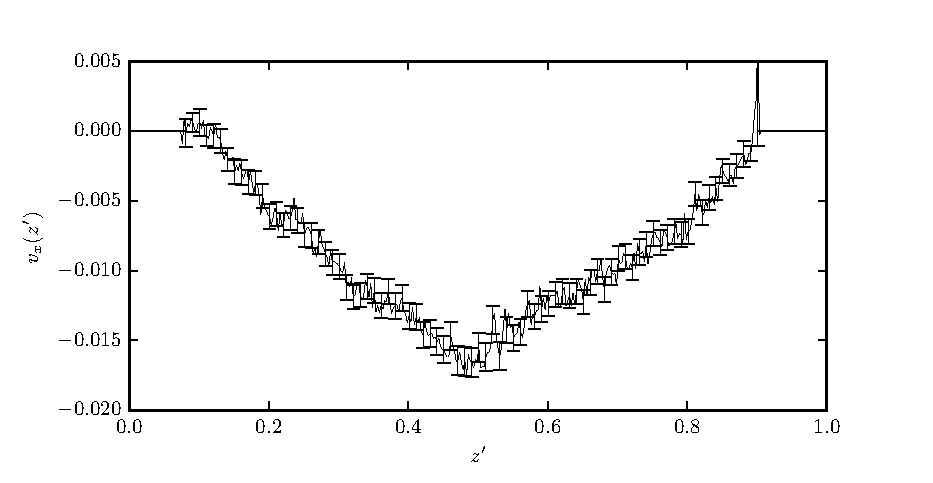
\includegraphics[scale=1.0]{PisVirFlow}
\caption{The velocity profile of a confined fluid at $T^{*}=0.85$ under the influence of the Virial Marangoni force was time--averaged over $40 \times 10^{6}$ timesteps of length $0.001\ \tau$.
A steady state negative interfacial peak emerges, corresponding to a Marangoni flow in the opposite direction to the temperature gradient.
The peak velocity magnitude is approximately 0.16 and this decays linearly to zero at the surface of the bounding walls, corresponding to a Couette flow.}
\label{PisVirFlow}
\end{figure*}
The fluid velocity profile is shown in Figure \ref{PisVirFlow}. 
There is a sharp negative peak at the interface indicating a Marangoni flow in the opposing direction to the temperature gradient.
Furthermore, the flow decays linearly away from the interface, consistent with a Couette flow arising from shear--driven fluid motion.\cite{FluidMech}

There is also a net flow in the system, suggesting an overall force acting on the fluid.
The walls in the system act as a momentum sink, providing a frictional force which allows this steady--state flow to arise under the isolated effect of a temperature--gradient.
\FloatBarrier

\subsubsection{Comparing to the Irving--Kirkwood stress}
Figure \ref{PisVirStress} shows the normal component of the Virial stress is not uniform across the interface.
In contrast, the normal stress calculated using the Irving--Kirkwood formula does not depend on the local fluid density and should therefore be constant throughout the liquid.
To verify if the difference in these methods has a significant effect on the measurement of the Marangoni force, the Irving--Kirkwood stress was also calculated.

\begin{figure*}[h]
\centering
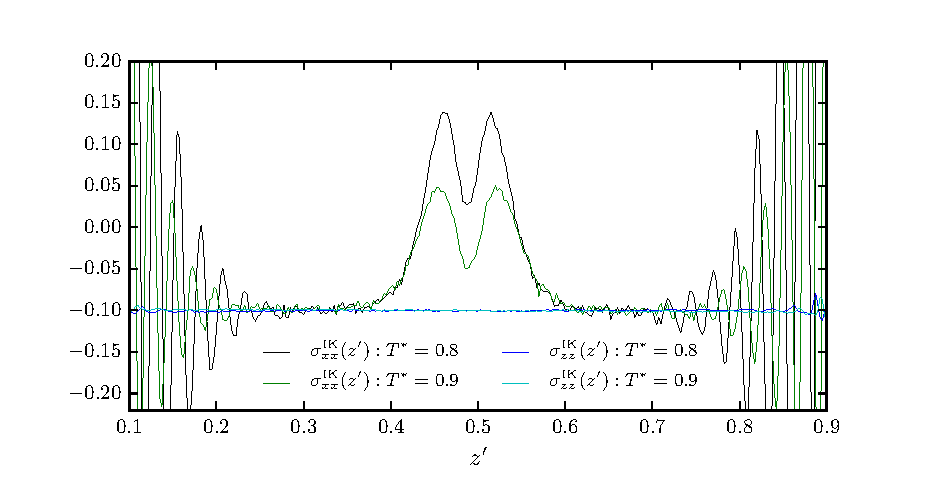
\includegraphics[scale=1.0]{PisIKStress}
\caption{The Irving--Kirkwood stress--tensor shows a similar profile to the Virial stress--tensor (see Figure \ref{PisVirStress}) although the interfacial peak is divided into two and a reduction in the stress occurs directly at the interface.
%This represents the reduction in the momentum flux across the interfacial plane as a result of the weaker interaction between non--equivalent fluid particles.
There are also similar oscillations at the wall due to a thermocapillary force.}
\label{PisIKStress}
\end{figure*}
\FloatBarrier
The fluids were prepared at $P^{*}=0.1$ and $T^{*}=0.8$ and $T^{*}=0.9$ as before.
Since the Irving--Kirkwood stress tensor was more computationally expensive (see Section \ref{CalcStress}), the equilibrium simulations were only run for $1 \times 10^{6}$ timesteps, resulting in a greater amount of statistical error.
This produced the time--averaged stress profiles shown in Figure \ref{PisIKStress}.
The tangential component of the Irving--Kirkwood stress shows a similar peak to the Virial stress whilst the normal component is constant throughout, as expected.
\FloatBarrier

\begin{figure*}[h]
\centering
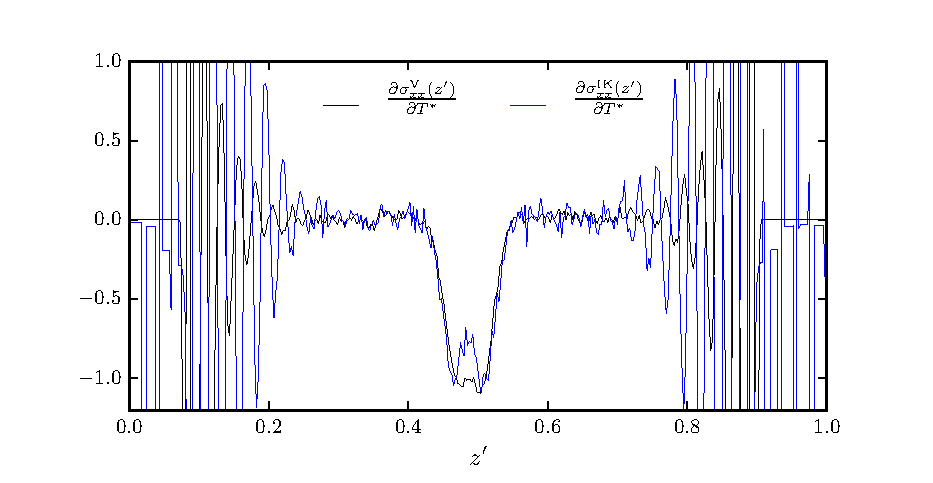
\includegraphics[scale=0.8]{PisIKForce}
\caption{The gradient of the Irving--Kirkwood stress--tensor with respect to temperature shows a peak across the interfacial region, representing the origin of the Marangoni force. This occurs with a similar maginitude to the gradient of the Virial stress--tensor although like the stress profile, the Irving--Kirkwood gradient is split into two peaks.
In both gradient profiles, there is no net gradient in the bulk and thus there will be no body force acting in the fluid bulk.}
\label{PisIKForce}
\end{figure*}
The finite difference method was again used to calculate the derivative of the stress with respect to temperature and this is compared to the Virial result in Figure \ref{PisIKForce}.
Still focussing on the central $1/3$ of the fluid, there is a good correspondence between the two derivatives and the interfacial peak occurs both across the same spatial region and with the same maximum value.
The most significant difference occurs directly at the interface, where there is a sharp reduction in the derivative of the Irving--Kirkwood stress.
This is probably a result of the reduction in density at the interface affecting the Virial stress--tensor more than the Irving--Kirkwood stress--tensor.
\FloatBarrier

\begin{figure*}[h]
\centering
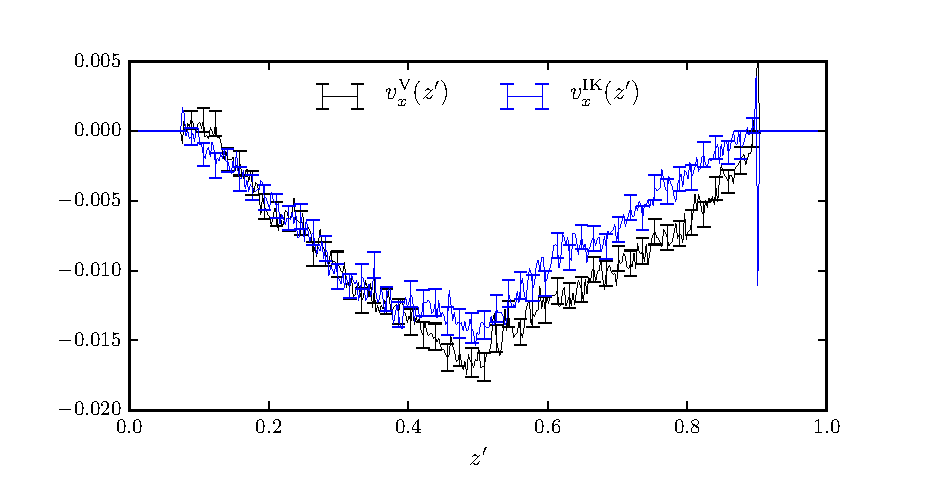
\includegraphics[scale=0.8]{PisIKFlow}
\caption{The flow profile calculated using the Irvining--Kirkwood Marangoni flow shows a similar profile to that calculated from the Virial force, with a sharp peak at the interface and a linear Couette flow into the bulk.
The peak value is not as large as that from the Virial force as a result of the sharp reduction of the Irving--Kirkwood stress gradient directly at the interface.
The Virial flow is symmetric whilst the Irving--Kirkwood flow is not, this is probably a result of the greater degree of noise in the Irving--Kirkwood gradient due to a short simulation time.}
\label{PisIKFlow}
\end{figure*}
Using a temperature gradient of $\partial T^{*} / \partial x^{*} = 0.001$ to compute the Irving--Kirkwood artificial body force, an equilibrium simulation at $T^{*} = 0.85$ was run for $40 \times 10^{6}$ timesteps.
The fluid velocity was measured and compared to the result obtained using the Virial force, as shown in Figure \ref{PisIKFlow}.
The profiles show a reasonably close correspondence, especially for the region $z' \leq 0.4$, although they deviate for higher values of $z'$.
In particular, the flow from the Irving--Kirkwood method is not as large directly at the interface, as a result of the reduction in the force at this point.
The Irving--Kirkwood velocity profile is also asymmetric despite the symmetry of the system.
This asymmetry may be the result of an increase in the noise of the Irving--Kirkwood force relative to the Virial force, which results from the shorter simulation time enforced by the high computational cost of the Irving--Kirkwood analysis.

\FloatBarrier
\subsection{Binary--mixture periodic in 3-dimensions}
Equation \ref{NavierStokes} demonstrated that the existence of a temperature gradient in the system should not be able to generate a net flow in the fluid. 
Levich discusses this further, describing how the interfacial flow must be accompanied by a back-flow in the bulk fluid.\cite{Levich}
In the case of the binary--mixture held between two walls, the stationary walls provide a momentum sink which allows a net flow to exist within the fluid.
To replicate the behaviour of an infinite fluid where a back flow may be observed, a system void of momentum sinks must be studied.
For example, a binary--mixture of two partially miscible fluids with periodic boundary conditions in all dimensions can be used.

This system, shown in Figure \ref{AABB}, was prepared as described in Section \ref{SystemPrep} with the parameters given in Section \ref{InteractionModel}.
The distance between consecutive interfaces was $0.5 L_{z^{*}}$.
A Nos\'{e}--Hoover barostat and thermostat were used to control the pressure at $P^{*} = 0.1$ with temperatures of $T^{*}=0.8$ and $T^{*}=0.9$.

\subsubsection{Comparing the Virial and Irving--Kirkwood stress}
There is again an ambiguity over which stress--tensor should be used for computing the Marangoni force.
Once equilibrated, the system was simulated for $10 \times 10^{6}$ timesteps over which the number density, Virial and Irving--Kirkwood stress were computed.
As discussed before, the Irving--Kirkwood analysis was computationally expensive and this simulation length was the upper feasible limit.
\FloatBarrier

\begin{figure}[h]
\centering
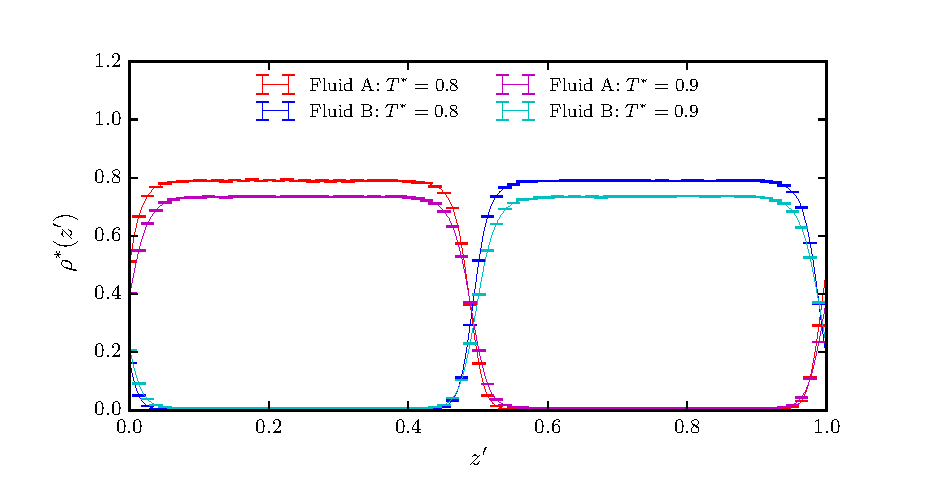
\includegraphics[scale=0.8]{Period10Rho}
\caption{The number--density of the component fluids at $T^{*}=0.8$ and $T^{*}=0.9$ shows a binary--mixture with the interface at around $z'=0.5$.
With the periodic boundary conditions, there are two interfaces per simulation box.
The number density falls at higher temperature and the position of the interface is slightly shifted, this shift must be removed before calculating the stress--gradient.}
\label{Period10Rho}
\end{figure}
After this period, the density profile (plotted in Figure \ref{Period10Rho}) showed a uniform density in the fluid bulk and a sharp interfacial region as expected.
However, the position of the interface shifted during the simulation and was no longer coincident for the two temperatures.
Before calculating the Marangoni force from the stress profile, this shift was removed by recentering the interfaces.
\FloatBarrier

\begin{figure}[h]
\centering
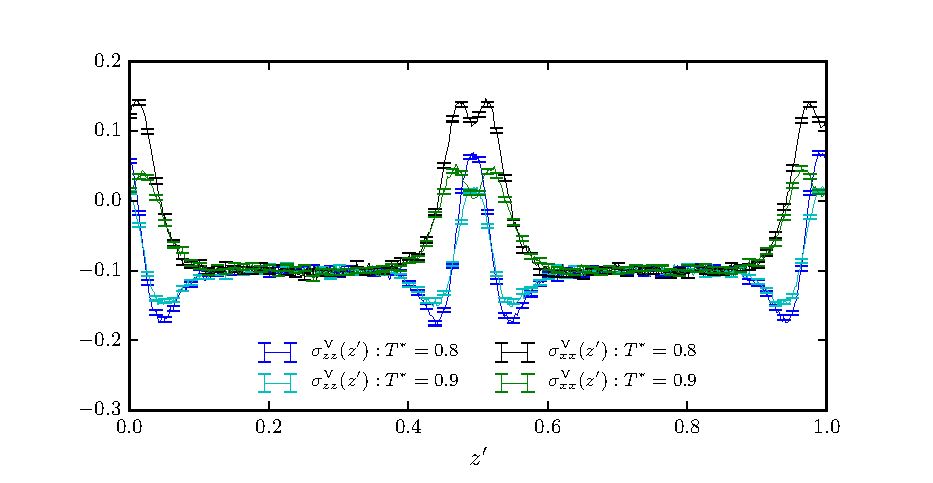
\includegraphics[scale=0.8]{Period10VirStress}
\caption{The tangential component of the Virial stress--tensor shows a bulk value of $-P_{ext}$ and a peak at the interfaces due to the anisotropy of the interparticle fluids at these points.
This peak has a similar form to that seen in the fluid confined between two wall, seen in Figure \ref{PisVirStress}.
}
\label{Period10VirStress}
\end{figure}

\begin{figure}[h]
\centering
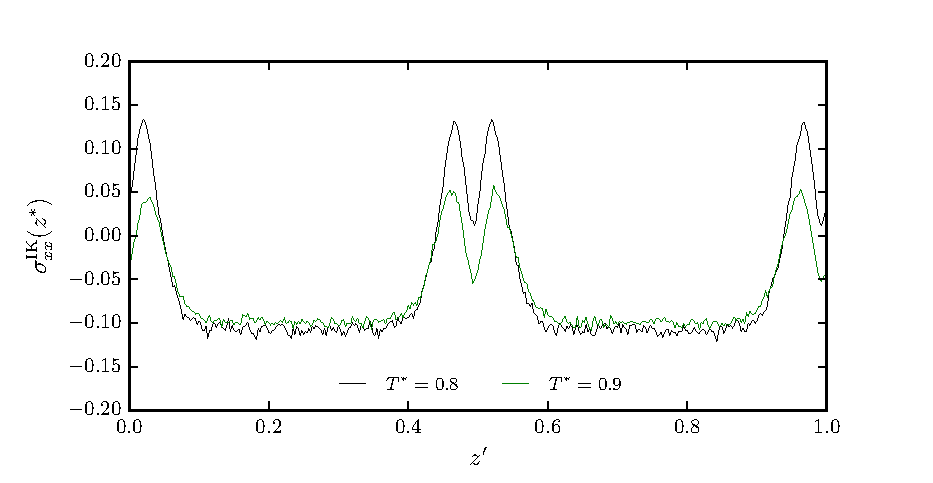
\includegraphics[scale=0.8]{Period10IKStress}
\caption{Similarly to Figure \ref{PisIKStress}, the Irving--Kirkwood stress for the binary--mixture periodic in three dimensions matches the Virial stress closely except directly at the interfaces.
The Irving--Kirkwood and Virial stress both show peaks of a similar magnitude and spatial coverage but the peak in the Irving--Kirkwood stress is again split into two peaks.
}
\label{Period10IKStress}
\end{figure}
The recentered Virial and Irving--Kirkwood stress profiles are plotted in Figures \ref{Period10VirStress} and \ref{Period10IKStress} respectively.
As with the fluid confined between two walls, the bulk stress components are equal to $-P_{\mathrm{ext}}$, corresponding to the hydrostatic fluid pressure.
There is an interfacial peak in both the Virial and Irving--Kirkwood tangential stress at the interface with a similar maximum value, although the Irving--Kirkwood stress shows a stronger minimum directly at the interface.
Similar to Figure \ref{PisIKStress}, this is probably the result of a reduced density in the interfacial region.
Furthermore, the normal component of the Irving--Kirkwood stress is clearly uniform across the interface, as expected.

\FloatBarrier
Using these stress profiles, the derivative of the stress with respect to temperature was calculated through the finite difference approach.
The derivative profile was adjusted by subtracting the average from each value, ensuring the integral over all space was zero, as shown in Figure \ref{Period10Force}.
This guaranteed there would be no net applied force acting on the fluid, even in the absence of a momentum sink in the system.

\begin{figure}[h]
\centering
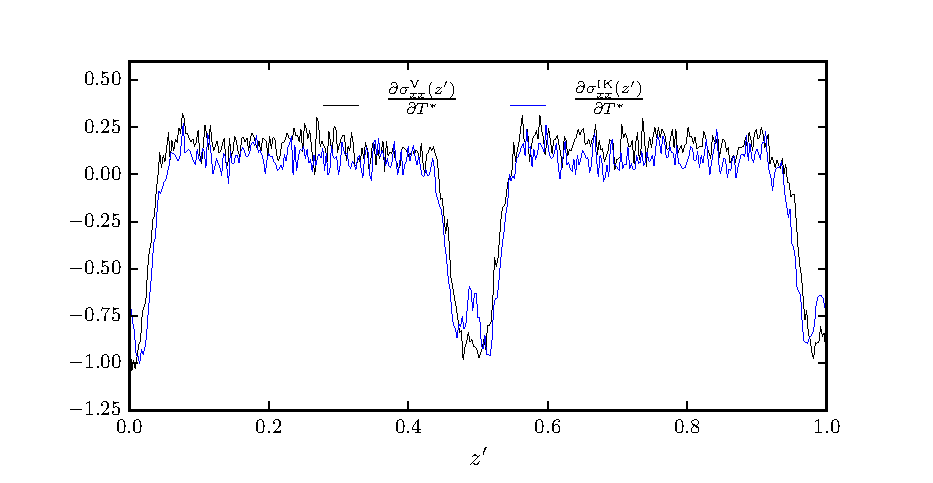
\includegraphics[scale=0.8]{Period10Force}
\caption{The gradient of the stress--tensor with respect to temperature calculated using equilibrium simulations of $10 \times 10^{6}$ timesteps shows the expected peak at the interfaces. 
This profile was adjusted to give no net gradient by subtracting the average gradient.
There appears to be a good correspondence between the Irving--Kirkwood and Virial stress--gradients, however such a short simulation timescale gives a large amount of noise in this gradient profile.
Consequently, the gradient profiles are not sufficiently precise to use for calculating an artificial body force and applying this to a non--equilibrium simulation.
}
\label{Period10Force}
\end{figure}
The derivative profile shows a similar interfacial peak to Figure \ref{PisIKForce}. 
The maximum values are similar, suggesting that fixing the total force to zero correctly adjusts the derivatives to give a physically meaningful Marangoni force.
Again there is a reasonably good correspondence between the derivatives calculated from the Irving--Kirkwood and Virial stress tensors, and the magnitude of the Irving--Kirkwood peak is reduced directly at the interface.
In the bulk fluid, the derivative opposes the interfacial peak, generating the back force which balances the Marangoni force.
However, the profile as a whole shows too much noise for the fine--structure to be determined and is not of sufficient quality to be used in calculating an artificial body--force.

\subsubsection{Reducing the noise in the force--profile}
To generate a profile with a sufficiently low noise requires either a larger system size or a longer simulation time.
Both of these increase the computational cost of calculating the Irving--Kirkwood stress beyond a practical level, and instead the Virial stress must be used.
Considering how similar the Virial and Irving--Kirkwood derivative profiles appear in Figure \ref{PisIKForce}, using the Virial stress does not create too much deviation from the more suitable Irving--Kirkwood stress, whilst enabling a much longer simulation time.
\FloatBarrier

\begin{figure}[h]
\centering
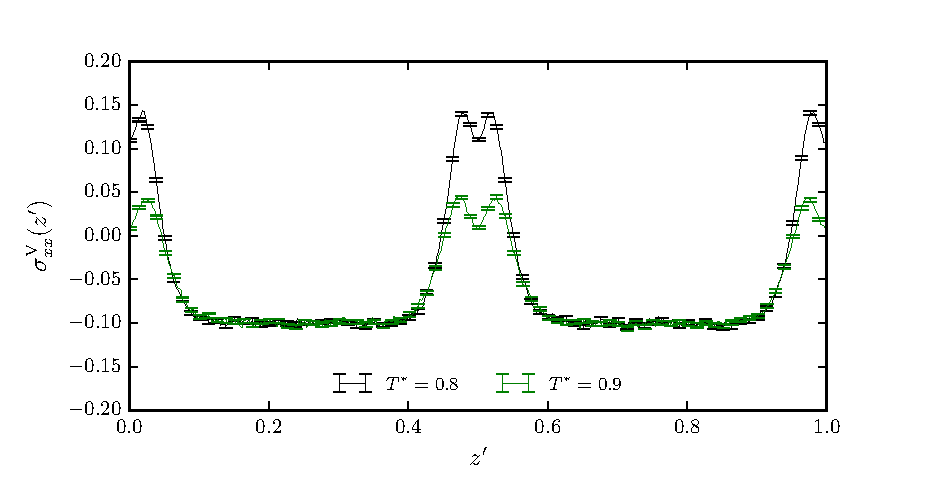
\includegraphics[scale=0.8]{Period30VirStress}
\caption{Running the equilibrium simulation over $30 \times 10^{6}$ timesteps produced a much more precise Virial stress profile with a significant reduction in noise relative to Figure \ref{Period10VirStress}.
The noise in the bulk stress lies within statistical error and thus is consistent with the hydrostatic pressure.
This simulation time is too long for the Irving--Kirkwood method to be feasible.
}
\label{Period30VirStress}
\end{figure}

The reduced noise stress was calculated by running the equilibrium systems for $30 \times 10^{6}$ timesteps.
Recentering the interfaces generated the Virial stress profile shown in Figure \ref{Period30VirStress}.
For both temperatures, the profiles show much less noise compared to Figure \ref{Period10VirStress}, especially in the bulk region, and the interfacial peaks are more symmetric.
\FloatBarrier

\begin{figure}[h]
\centering
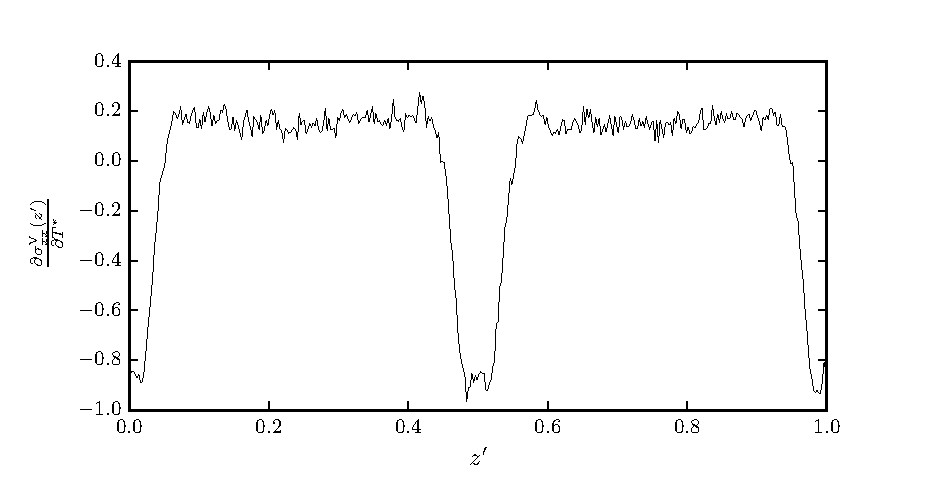
\includegraphics[scale=0.8]{Period30VirForce}
\caption{The Virial stress gradient calculated using equilibrium simulations of $30 \times 10^{6}$ timesteps showed significantly less noise than the equilibrium simulations of $10 \times 10^{6}$ timesteps.
Having subtracted the average value, the plot confirms there is a sharp and symmetric interfacial peak with an opposing bulk derivative.
}
\label{Period30VirForce}
\end{figure}

Using these stress profiles, the derivative of the stress--tensor with respect to temperature was again computed using the finite difference and the average value subtracted to give the profile shown in Figure \ref{Period30VirForce}.
There is a dramatic reduction in the noise compared to Figure \ref{Period10Force}, with a sharp peak at the interface and an opposing stress derivative in the bulk regions.
\FloatBarrier

Using the stress derivative given in Figure \ref{Period30VirForce} and a temperature gradient of $\partial T^{*} / \partial x^{*} = 0.001$, an artificial body force was computed.
The body force was recentered to ensure the Marangoni peak was aligned with the interfacial region, and this was applied in an equilibrium simulation at $T^{*} = 0.85$.
This simulation was run for $40 \times 10^{6}$ timesteps, and $v^{*}_x(z')$ was computed to give the flow velocity plotted in Figure \ref{Period30VirFlow}.

\begin{figure}[h]
\centering
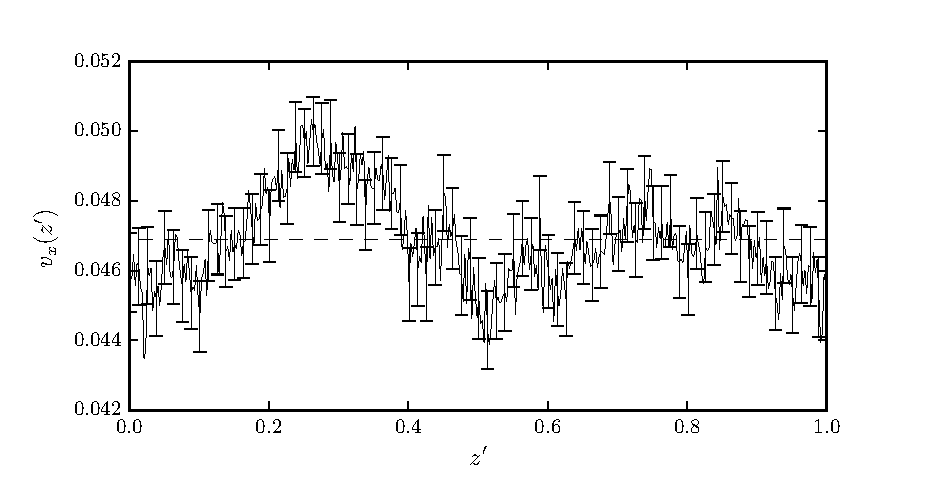
\includegraphics[scale=0.8]{Period30VirFlow}
\caption{The flow profile calculated from a non--equilibrium simulation using the stress gradient shown in Figure \ref{Period30VirForce} and a temperature gradient of $\partial T^{*} / \partial x^{*} = 0.001$ has a large amount of noise and is not very conclusive.
There is a net flow velocity despite the average gradient being set to zero, it is unlikely this could be improved upon without artificially fixing the centre--of--mass.
Despite this, the fluid velocity relative to this centre--of--mass motion suggests a negative peak at the interfaces with some back flow in the bulk regions, satisfying Levich's requirement of a stationary net flow.\cite{Levich}
 }
\label{Period30VirFlow}
\end{figure}

Despite the simulation being run for a long timescale, the velocity profile still retains a lot of statistical noise.
It would be difficult practically to reduce this noise further.
Moreover, the average velocity (indicated by the hashed line) is non--zero, indicating centre--of--mass motion during the simulation.
This motion occurs even though the stress derivative has been adjusted to give no net force overall.
It is likely that in the absence of a momentum sink for a system like this, it would be very difficult to completely remove this net flow without artificially fixing the centre--of--mass throughout the simulation.

Despite this, the relative motion across the fluid can still be considered, and there does appear to be a velocity peak at the interface (with $v < v_{\mathrm{COM}}$), corresponding to a Marangoni flow, with a back flow in the bulk fluid (with $v > v_{\mathrm{COM}}$) as predicted.
This result is, however, somewhat ambiguous and there was insufficient time to improve this simulation further.

\subsection{The effect of surfactants}\label{SurfResult}
Surfactant molecules decrease the surface free energy of interfaces, as they have a favourable interaction with both fluids and bridge the interfacial plane.
This reduction in surface tension should also cause a decrease in the surface tension gradient and thus the Marangoni effect, as observed experimentally.\cite{KimSubramanianA,KimSubramanianB,BartonSubramanian,ChenStebe}

To model this, the non--ionic surfactant molecules described in Section \ref{ModellingSurfactants} were added to the binary--mixture confined between two walls.
This system was chosen since the results of Section \ref{Piston} showed it allowed a steady state flow to be generated and modelled effectively.

The surfactant molecules were added to a single plane between the two fluids in the initial lattice before melting.
A certain fraction of these molecules were then removed to vary the surfactant concentration, quantified as a fraction of the total number of fluid particles present,
\begin{equation}
\mathrm{Surfactant\ Fraction} \equiv \frac{N_{\mathrm{surfactant}}}{N_{\mathrm{surfactant}}+N_{\mathrm{fluid}}}.
\end{equation}
This allowed the surfactant fraction to be varied between $0$ and $0.0323$.

Taking fractions of $0.000$, $0.0031$, $0.0098$, $0.0194$, $0.0264$, $0.0298$ and $0.0323$, the fluid was prepared as described in Section \ref{SystemPrep}, with a pressure of $P^{*}=0.1$ and temperatures of $T^{*}=0.8$ and $T^{*}=0.9$.
A piston barostat and Nos\'{e}--Hoover thermostat were used and each system was run at equilibrium for $30 \times 10^{6}$ timesteps of length $0.001\ \tau$.

\begin{figure}[h]
\centering
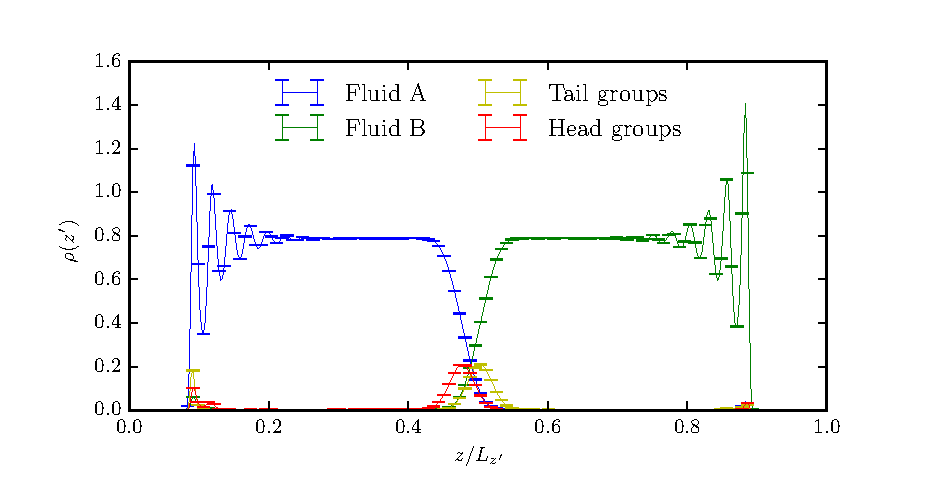
\includegraphics[scale=0.8]{SurfRho}
\caption{The number density for the binary--mixture with nonionic surfactant molecules, at  $T^{*}=0.8$ and with a surfactant fraction of $0.0194$, is plotted.
There is a uniform density in the bulk, showing a fluid like state, and a sharp interface where the densities of Fluid A and Fluid B change rapidly.
The surfactant particles are localised at the interface with a low solubility.
They also show the correct orientation, with `Head' particles interacting most strongly with Fluid A and `Tail' particles with Fluid B.
}
\label{SurfRho}
\end{figure}

The resulting number density of each species shows a uniform bulk density, a sharp interface and peaks for the head and tail groups located at the interface, as shown for $T^{*}=0.8$ and a surfactant fraction of $0.0194$ in Figure \ref{SurfRho}.
The surfactant molecules were correctly oriented with head groups interacting with Fluid A and tail groups with Fluid B.
\FloatBarrier

\begin{figure}[h]
\centering
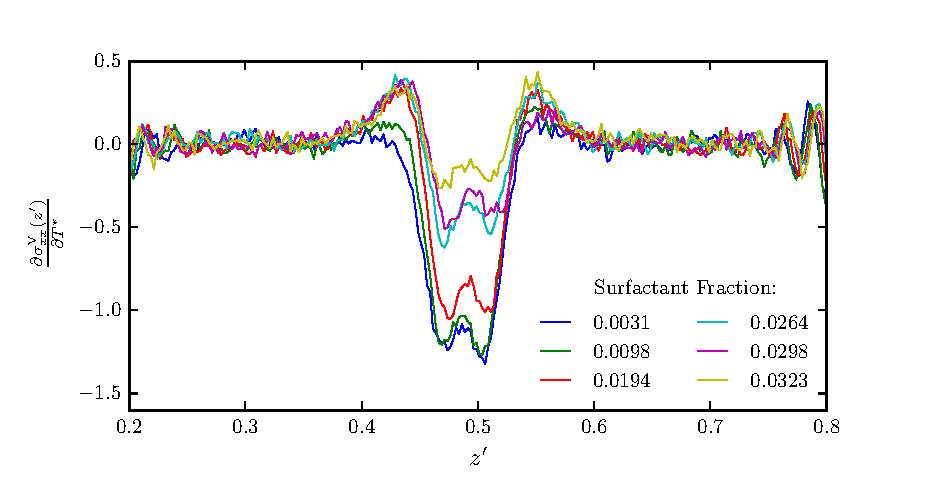
\includegraphics[scale=0.8]{SurfForce}
\caption{The gradient of the Virial stress--tensor for the surfactant systems still shows a strong interfacial peak for a low surfactant fraction.
As the amount of surfactant is increased, the strength of this peak decreases to zero with a resulting reduction in the Marangoni force.
}
\label{SurfForce}
\end{figure}

The Virial stress was computed during the equilibrium simulations and used to compute the derivative of the stress with respect to temperature for each surfactant fraction.
These results, plotted in Figure \ref{SurfForce}, show a pronounced reduction in the magnitude of the interfacial peak as the surfactant fraction increases, corresponding to the expected reduction in the Marangoni force.

Two smaller positive peaks on either side of the centre also develop for higher surfactant fractions.
It is unclear exactly what these peaks correspond to.
They may simply be the result of an increase in the fluid density, due to localisation of the surfactant particles in this region and the dependece of the Virial stress on local density.
An increase in surfactant fraction would then exaggerate this density change.
In future, this could be verified by computing the Irving--Kirkwood stress, where any peaks due to density deviations should disappear.

Furthermore, the harmonic forces in the surfactant molecules may provide a contribution to these peaks in the stress.
The physical significance of this contribution could be investigated by varying the spring constant for the surfactant bond and noting any changes in the magnitude of these secondary peaks.
\FloatBarrier

\begin{figure}[h]
\centering
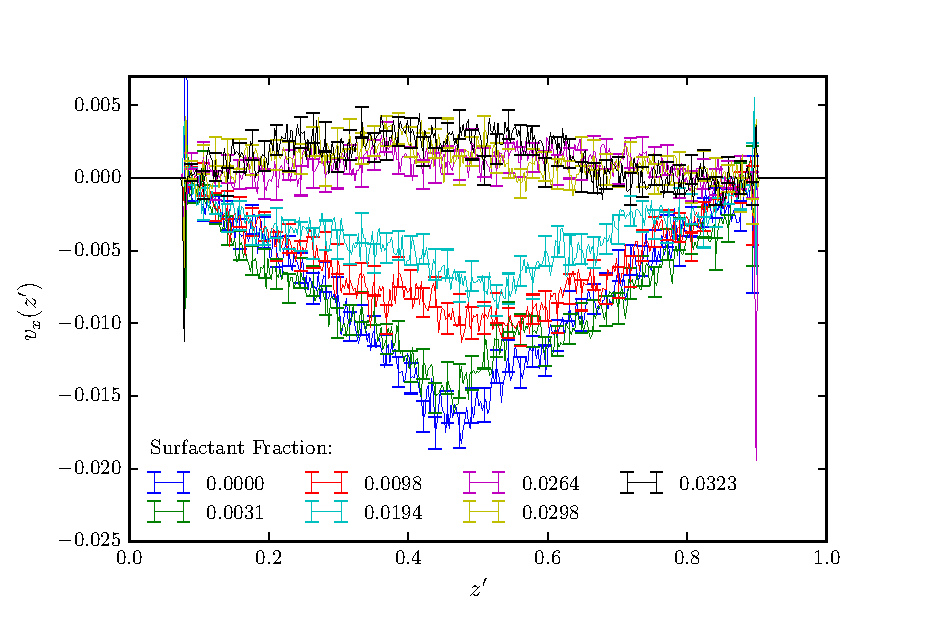
\includegraphics[scale=0.8]{SurfFlow}
\caption{For a low surfactant fraction, the flow profile closely resembles that of the non--surfactant system with an interfacial peak and a linear decay into the bulk.
As the amount of surfactant increases there is a reduction in the magnitude of this peak until the Marangoni flow is essentially removed.
}
\label{SurfFlow}
\end{figure}
Using a temperature gradient of $\partial T^{*} / \partial x^{*} = 0.001$, the central $1/3$ of the stress derivative profiles in Figure \ref{SurfForce} were used to compute an artificial body force, which was applied to simulations at $T^{*}=0.85$.
These were run for $30 \times 10^{6}$ timesteps over which $v_{x}(z')$ was measured and plotted in Figure \ref{SurfFlow}.
There is a clear decrease in the interfacial velocity as the surfactant fraction is increased, suggesting a retardation of the Marangoni effect induced by the surfactant molecules.

\FloatBarrier
\begin{figure}[h]
\centering
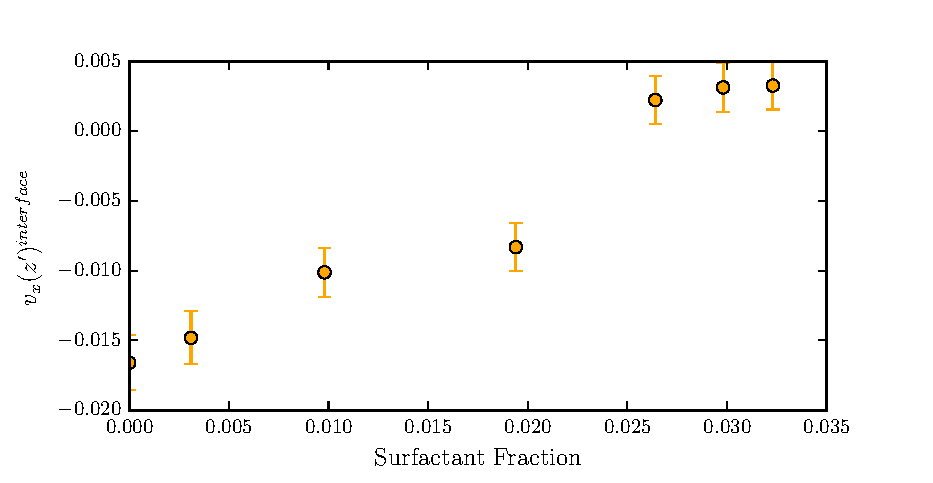
\includegraphics[scale=0.8]{InterVel}
\caption{As the surfactant fraction in the system increases, the magnitude of the interfacial velocity decreases.
Above a fraction of $0.025$, this velocity is essentially zero, although there is small velocity in the opposite direction to the Marangoni flow.
This backwards velocity may be the result of a gradient in the amount of surfactant at the interface, which could occur as the surfactant molecules will be more soluble at higher temperatures so will have a smaller interfacial excess.
Such an effect may only be significant for high surfactant concentrations.
}
\label{InterVel}
\end{figure}
The interfacial velocity can be taken as the peak of the flow shown in Figure \ref{SurfFlow}.
Comparing these values against the surfactant fraction shows a reduction in the magnitude of this peak value as the surfactant fraction increases, as shown in Figure \ref{InterVel}.
Above a fraction of $0.025$ it appears the Marangoni effect has been removed completely.
This retardation has been observed experimentally by Barton and Subramanian and is discussed in their study on the relation between droplet size and upward motion under a vertical temperature gradient.\cite{BartonSubramanian} 
They note that droplets actually sink on the addition of a nonionic surfactant, indicating the eradication of the Marangoni force and the dominance of gravity.

\FloatBarrier
The sharpness of the Marangoni flow peak in Figure \ref{SurfFlow} also decreases as the surfactant fraction increases and no longer fits the Couette model as conclusively.
This may be a result of the reduction in viscosity at the interface due to the presence of surfactant molecules, giving a non-uniform viscosity across the fluid. 
To confirm this, the viscosity could be measured using the Green--Kubo relation,
\begin{equation}
\eta = \frac{1}{V k_{\mathrm{B}} T} \int_{0}^{\infty} \left< \sigma_{xy} \left( \tau \right) \sigma_{xy}(0) \right> \mathrm{d} \tau,
\end{equation}
providing a good basis for future work in this area.

\newpage
\section{Concluding Remarks}
Using equilibrium simulations at two close temperatures, the derivative of the tangential component of the stress tensor with respect to temperature was estimated for binary--mixtures through a finite--difference method.
The derivatives of the Virial and Irving--Kirkwood stresses were calculated for a mixture confined between two walls, and in both cases there was a similar negative interfacial peak.
Combining with a temperature gradient, an artificial body force was computed and applied in a third equilibrium simulation, resulting in a non--equilibrium with a net interfacial flow.
This was interpreted as a Marangoni flow and occurred in the opposite direction to the applied temperature gradient, as expected.
The confining walls provided a momentum sink in the system, exerting a frictional force on the fluid and allowing a steady state flow to be achieved.

The same method was then applied for a binary--mixture periodic in all dimensions, and a similar peak in the stress derivative was observed.
However, the fine structure of this derivative was obscured by significant noise.
This was reduced by running the simulation for a longer time period.
As a result, only the Virial stress was feasible for calculating a sufficiently precise gradient profile.

In the absence of a momentum sink, the stress derivative was adjusted to ensure no net force was applied on the system, and was used to calculate an artificial body force.
Applying this force produced a flow profile showing a negative peak at the interfaces relative to a net centre--of--mass motion, and an associated back flow in the bulk of the fluid.

The origin of the centre--of--mass motion is unclear. 
It is possible, although unlikely, that is is the result of errors induced by noise in the applied force.
For example, errors in the average derivative will cause the derivative profile to be incorrectly recentred, and a net applied force could result.
Running the initial equilibrium simulations for an even longer period could allow a more precise force to be calculated and the effect of noise verified. 

Alternatively, the centre--of--mass could be artificially held stationary throughout the simulation.
However, this would be rather unphysical, since observing a stationary centre--of--mass is essential to verifying the correct behaviour of Maragnoni flows.
Fixing the centre--of--mass would allow only the relative motion of different fluid regions to be observed.

Having established a working system in the form of the fluid confined between two walls, the effect of surfactants on Marangoni flows was investigated by adding different concentrations of non-ionic surfactant molecules into the interfacial region.
The tangential Virial stress was again computed at two temperatures and its derivative with respect to temperature was estimated through the finite difference.
As the concentration of surfactant increased, there was a reduction in the magnitude of the negative interfacial peak and the emergence of two secondary positive peaks on either side of the interface..

The stress derivatives were used to calculate an artificial body force that was then applied in a third equilibrium simulation.
The magnitude of the resulting Marangoni flow was seen to decrease to zero as the surfactant concentration increased, in agreement with experimental studies.
Furthermore, the shape of the velocity profile deviated from the linear decay observed in the absence of surfactant.
This may be due to a non--uniform fluid viscosity, since the addition of surfactants should decrease the viscosity of the interfacial region.

\subsection{Future directions of study}
There are a number of ambiguities in the results reported which may be verified through further study.
For example, if more time was available it would be interesting to compute more accurate force profiles from the Irving--Kirkwood stress by using a larger system.
This could be made more efficient by implementing the Irving--Kirkwood analysis in parallel.

Furthermore, by introducing a contribution from the harmonic bonding into this analysis, it could be used to study systems with added surfactant.
Using the Irving--Kirkwood stress would confirm whether the secondary peaks observed as surfactant fraction increases are the result of an increase in local density due to the presence of surfactant particles, or some other significant physical feature.

It would also be interesting to compute the viscosity across the liquid and compare this for the pure fluid and the fluid with surfactant present.
As described in Section \ref{SurfResult}, this can be calculated using a Green--Kubo relation.
Comparing the shape of the flow profile to the uniformity in the viscosity would allow the deviation from the Couette flow model to be investigated.

Beyond this, linear response theory suggests that the flow induced by a temperature gradient could computed as:
\begin{equation}
\left< v_{x} \right> = \frac{\nabla T}{T} V \int_{\tau =0}^{\infty} \left< J_{x}(0) Q_{x}(\tau) \right> \mathrm{d} \tau,
\label{LinResponse}
\end{equation}
where $J$ and $Q$ are the mass and heat flux respectively.
By computing this average velocity for the mixture confined between two walls, both with and without an applied body force, Equation \ref{LinResponse} could allow a general relation between flow velocity and temperature gradient to be developed.
This could be compared for the bulk and interfacial regions, since there should be no correlation between the heat flux and mass flux away from the interfaces.

In addition to this, a greater understanding could be developed using Onsager's reciprocal rule, as employed be Derjaguin et al.
This could be achieved by applying a pressure gradient to a simulation and measuring the resulting heat flux.
From the relation of these quantities, the mass flux from a temperature gradient could be computed. 

Finally, once informative methods for the basic study of Marangoni flows have been developed, the natural progression would be to investigate different systems and geometries.
For example, it would be interesting to study a non--symmetric binary--mixture or to replicate the thermophoresis of bubbles and drops under a temperature gradient, as observed experimentally.
\\
\\
\indent Through the results of this study, combined with future work, a greater understanding of the relationship between the stresses within a fluid and the velocity due to a temperature gradient can be achieved. 
Ultimately this is working towards a microscopic description and a more comprehensive understanding of the Marangoni effect.




\newpage
\addcontentsline{toc}{section}{Bibliography}
\bibliography{dissertation_master}
%\thispagestyle{empty}
\newpage
\cleardoublepage

\end{document}
